\documentclass[9pt,conference]{IEEEtran}
\usepackage[nomarkers]{endfloat}
\usepackage[cmex10]{amsmath}
\usepackage{filecontents}
\usepackage{lipsum}
\usepackage{graphicx}

\begin{filecontents*}{informe.bib}
@electronic{refmallba,
  author        = {Universidad de M\'alaga},
  title         = {Referencia Mallba/Malva},
  url           = {http://neo.lcc.uma.es/mallba/easy-mallba/index.html},
  year          = {2008}
}
@electronic{refwmaker,
  author        = {Daniel W. Dyer},
  title         = {Referencia Watchmaker},
  url           = {http://watchmaker.uncommons.org},
  year          = {2006}
}
\end{filecontents*}

\begin{document}

%-------- Metadata -------- 
	\title{Pr\'actico 1}
	\markboth{Algoritmos Evolutivos 2015}{Shell \MakeLowercase{\textit{et al.}}: A Novel Tin Can Link}
	\author{
		\IEEEauthorblockN{Gonzalo Torterolo}
		\IEEEauthorblockA{
			Facultad de ingenier\'ia\\
			UDELAR\\
			Montevideo, Uruguay\\
			Email: gonzalo.torterolo@fing.edu.uy
		}
		\and
		\IEEEauthorblockN{Gisel Cincunegui}
		\IEEEauthorblockA{
			Facultad de ingenier\'ia\\
			UDELAR\\
			Montevideo, Uruguay\\
			Email: gisel.cincunegui@fing.edu.uy
		}
	}



% ------- Contenido -------
	\maketitle

	\begin{abstract}
	En el presente informe el objetivo es probar las ventajas y limitaciones de las actuales librerias que implementan algoritmos gen\'eticos mediante la resoluci\'on de 2 problemas t\'ipicos de computaci\'on. Adem\'as se realizan pequeños analisis de las soluciones con el fin de verter conocimientos te\'oricos adquiridos en el curso.
	\end{abstract}
	\begin{IEEEkeywords}
	Algoritmos Evolutivos, AE, Algoritmos Gen\'eticos, AG, Malva, Mallba, Whatchmaker, Knapshak, Mochila
	\end{IEEEkeywords}

	\section{Introducci\'on}
	En la consigna presentada (ver letra en \cite{refmallba}) se deben resolver dos variantes del problema de la mochila (explicadas en la consigna tambi\'en) utilizando ideas de los algoritmos gen\'eticos.

	Por otra parte, el an\'alisis y modelado del problema as\'i como las ventajas de utilizar este tipo de algorimos para el escenario queda relegado a una segunda instancia, pues ya estaban resueltos en las consignas. En todo momento prim\'o la aplicaci\'on de los conceptos te\'oricos del curso antes que la obtenci\'on de resultados como rendimiento, modularidad, etc. No nos interesa, por lo tanto, seguir aqu\'i un enfoque pr\'actico para esta primer aproximaci\'on a los algoritmos evolutivos donde ambos problemas son t\'ipicos y ampliamente estudiados.


	\subsection{Aplicaci\'on de AG}

	Se analizan las diferentes soluciones a las dos variantes del problema de la mochila aqu\'i presentadas, concluyendo con una implementaci\'on para ambos casos.
	Para comenzar a definir las soluciones a los problemas se debe determinar las siguientes car\'acter\'izticas de importancia para un AE t\'ipico.

	\begin{enumerate}
		\item Codificaci\'on.
		\begin{itemize}
				\item Tratamiento de codificaciones no factibles.
		\end{itemize}
		\item Poblaci\'on inicial.
		\begin{itemize}
				\item  Evaluaci\'on de coste/beneficio de utilizar criterios inteligentes de inicializaci\'on.
				\item  Velocidad de convergencia a un \'optimo.
		\end{itemize}
		\item Funcion de fitness.
		\begin{itemize}
				\item  Car\'acter\'izticas especiales requeridas (e.g.: no negatividad de la funci\'on para selecc\'ion proporcional)
				\item  Transformaci\'on para otros escenarios (e.g.: aplicaci\'on para maximizaci\'on/minimizaci\'on)
				\item  Ajustes para mejorar soluciones (escalado, par\'ametros de configuraci\'on).
		\end{itemize}
		\item Seleccci\'on:
		\begin{itemize}
				\item  Elitismo o no.
		\end{itemize}
		\item Cruzamiento.
		\begin{itemize}
			\item Definir operadores de cruzamiento y estudiar la deriva gen\'etica que estos puedan provocar. 
		\end{itemize}
		\item Mutaci\'on.
		\begin{itemize}
			\item Definir operadores de mutaci\'on. 
		\end{itemize}
	\end{enumerate}

	\subsection{Particularidades y observaciones de las implementaci\'on/Librerias}
	\begin{itemize}
		\item Malva
		\begin{itemize}
			\item Malva utiliza otro concepto para la mutaci\'on, la probabilidad se aplica por individuo y no por gen.
			\item Parece bastante desprolija, aunque quiz\'as mucho m\'as performante y escalable que cualquier otra, pero como ya se dijo, estas car\'acter\'izticas no interesan en este momento.
		\end{itemize}

		\item Whatchmaker
		\begin{itemize}	
			\item Permite elitismo y esta cantidad es extra a la de la poblaci\'on especificada.
			\item Es bastante menos performante que Malva, pero consisten en una estructura mucho m\'as ordenada y flexible, por la que la preferimos a la hora de prototipar nuestra implementaci\'on.
		\end{itemize}
	\end{itemize}

	\subsection{Problemas de los aperitivos}
	
	Para este primer problema interesa obtener el \'optimo de un problema. La aplicaci\'on de AE no nos parec\'io muy adecuada, pues no se estaba buscando una soluci\'on aceptable, sino que solo la mejor soluci\'on posible es aceptable para los comensales. Por otra parte, el problema es multimodal y NP computacionalmente dificil, lo que lo hace atractivo a una soluci\'on de AG.
	En esta variante del problema de la mochila se buscan soluciones enteras pero se aceptan repeticiones, y no existen pesos, o puede entenderse que el peso es proporcional a la ganancia o costo (es el mismo).
	Se utiliz\'o la liber\'ia Malva en este problema.
	Se definen las caracterizticas de la soluci\'on relativas al AG:

	Notaci\'on
		$$X_i,C_i$$\\ son la cantidad de aperitivos, costo de aperitivo para el tipo $i$ respectivamente\\
		$$N,O$$\\ la dimensi\'on del problema y costo objetivo respectivamente\\

	\begin{enumerate}
		\item Codificaci\'on.
		Nos es importante utilizar una codificaci\'on conveniente a para facilitar el trabajo del cruzamiento y utilizar SPX o cruzamiento uniforme que ya se encuentran implementadas.

		\item Evaluamos la posibilidad de utilizar 2 tipos de codificaciones.
			La primera de ella muy parecida a la pedida en el pr\'oximo problema, donde asignamos un gen binario (los alelos toman valores en \{0,1\}) para cada posible aperitivo en caso de que se elija o no. En el caso deber\'iamos asignar una cota a la cantidad del genoma, dada por \ref{eq_tope_rep} para cada tipo de aperitivo. Esta codificaci\'on es bastante intuitiva pero tiene la desventaja de asignar varios genotipos a un mismo fenotipo. El cruzamiento SPX tiene un comportamiento menos discruptivo en esta representaci\'on. Podr\'ia ser \'util en etapas avanzadas de la evoluci\'on.

			\begin{equation}
			\label{eqn_tope_req}
			M_i = \lceil \frac{N}{C_i} \rceil
			\end{equation}

			Otra codificaci\'on elimina el problema de que varios genotipos se correspondan con un mismo fenotipo. La misma consite en una representaci\'on de enteros, donde cada gen representa la cantidad de aperitivos de un tipo dado. Aplicada junto a un cruzamiento SPX esta codificaci\'on tiene un comportamiento m\'as discruptivo que la anterior, se mueve por bloques.

			Se puede incluso, utilizar ambas representaciones en distintas etapas de la evoluciones, de hecho propondremos una funci\'on de fitness que es {compatible} para ambas codificaciones.

			En las codificaciones anteriores se le puede agregar sem\'antica en el ordenamiento del cromosoma. Se discute la posibilidad de ordenar los genes dentro del cromosoma en funci\'on del costo.

			Para la implementaci\'on se elige la segunda opci\'on, sin agregar informaci\'on en el ordenamiento.
		
		Todas las soluciones representables ser\'an consideraciones factibles.

	\item Selecci\'on
		Usaremos selecci\'on proporcional tanto para la selecci\'on de cruzamiento como selecci\'on generacional, ya implementada en malva utilizando el algoritmos de la ruleta. La funci\'on de fitness toma valores positivos, por lo que es adecuada para este tipo de selecci\'on.

	\item Fitness
		Tomaremos como funci\'on de fitness la distancia al valor objetivo.
		Podemos configurar la librer\'ia Malva para resolver un problema de minimizaci\'on en vez de maximizaci\'on, por lo que no hace falta transformar la funci\'on de fitness.
		\[ v = |\sum\limits_{i=0}^{N} (C_i X_i) - O| \]
		es la distancia del valor objetivo.

	\item Cruzamiento
		Se ha enfocado la elecci\'on de las anteriores caracter\'izticas de AG para utilizar SPX, pero otros algoritmos de cruzamientos donde se apliquen operadores num\'ericos podr\'ia surgir, como por ejemplo, se propone el promedio entre valores de cada padre, o diferentes promedios ponderados. Sin embargo, para la implementaci\'on se opta por SPX.

	\item Mutaci\'on
		Se utiliz\'o una mutaci\'on uniforme sobre los valores posibles de alelo de cada gen, expresada por la formula:
		\[ X_i = (X_i + rand(0,M_i)) \% M_i \]


	Poblaci\'on inicial
		La poblaci\'on inicial ser\'a muy importante para determinar una buena soluci\'on, pues a partir de ella se tiene casi todo el material gen\'etico nuevo. En las ejecuciones donde se ha probado la probabilidad de mutaci\'on baja hace que no se genere nuevo material gen\'etico m\'as del aportado por la poblaci\'on inicial. Sin embargo, una cantidad suficiente de individuos en cada generaci\'on logra cubrir el espacio de busqueda bastante bien. Para la generaci\'on de la poblaci\'on inicial se utiliz\'o un criterio aleatorio, pero se asegura que existen al menos un aperitivo de cada tipo al asignar el m\'aximo valor factible a en alg\'un gen de cada individuo (el gen numero de individuo \% cantidad de genes del cromosoma).
	\end{enumerate}

	\subsection{Problemas de la mochila}


	\begin{itemize}	
	\item Descripcion del problema:
		El problema es un problema de optimizaci\'on combinatoria perteneciente a la familia de problemas N-P dif\'iciles. El problema se define de la siguiente manera:
		Dados un conjunto de n objetos, cada uno con una ganancia asociada gi y un peso asociado pi, el objetivo del problema es encontrar el subconjunto de objetos que maximiza la ganancia total, manteniendo el peso total por debajo de la capacidad m\'axima de la mochila (W). En ecuaciones ver \ref{eqn_tot_gain} y \ref{eqn_tot_peso}:
		\begin{equation}
		\label{eqn_tot_gain}
		G_{tot} = \sum\limits_{i=0}^{n} g_{i}x_{i}
		\end{equation}

		\begin{equation}
		\label{eqn_tot_peso}
		P_{tot} = \sum\limits_{i=0}^{n} p_{i}x_{i} < W
		\end{equation}

	
	\item Descripci\'on de la soluci\'on:
			Este problema constiste en obtener una soluci\'on lo mas pr\'oxima posible a la \'optima del problema, implementando para ello t\'ecnicas de algoritmos evolutivos.
			A continuaci\'on se detallar\'a las desiciones para la implementaci\'on del algoritmo evolutivo del problema de la mochila:
	\end{itemize}	
	\begin{enumerate}
	
	\item Codificacion:
		\begin{itemize}	

		\item Arreglo binario con el largo igual a la cantidad de elementos totales que puedo incorporar en la mochila, donde cada posicion del arreglo correspone a el objeto $i$ de la soluci\'on. Dicho arreglo ser\'a ordenado por peso, manteniendo la referencia del ordenamiento del arreglo original, ya que se busca con esto que la operacion de cruzamiento operada por el algoritmo evolutivo intente probar distintos valores de ganancia ``manteniendo'' relativamente el peso de la solucion mas factible.
		El odenamiento de el arreglo se har\'a manteniendo dos estructuras de indices para la codificacion (arreglo original -> arreglo ordenado , fenotipo -> genotipo) y la decodificacion (arreglo ordenado -> arreglo original, genotipo -> fenotipo).
		La funci\'on de fitness se evaluar\'a con el fenotipo, las operaciones se realizaran con el genotipo, y el resultado retornar\'a el fenotipo de la mejor solucion encontrada.

		\item Factibilidad de la solucion:\\ 
			Se tomar\'a como solucion factible aquella que no sobrepase el limite de peso de la mochila.
		\end{itemize}	
			
	\item Poblaci\'on inicial:\\
		\begin{itemize}	
		\item Para la poblaci\'on inicial se opt\'o por la generacion aleatoria de los individuos, pues podemos ver que en varias ejecuciones se alacanza r\'apidamente un \'optimo del problemas.
		\end{itemize}	
		
	\item Funcion de fitness:\\
			La ecuacion final de la misma ha mutado de acuerdo a problemas que se nos han planteado a lo largo de la implementacion. Al principio se opt\'o por lo siguiente:	
		\begin{itemize}	
			\item Funcion con penalizacion:\\
			La idea de esta funci\'on es mantener los individuos no factibles a lo largo de las generaciones para evitar la deriva gen\'etica, ya que los mimos pueden brindar informacion relevante para llegar a la optimizacion de la solucion final.
			Si el peso total del individo no sobrepasa al max\'imo permitido para la mochila(candidato factible), la funci\'on de fitness retornar\'a la ganancia total del individo evaluado.
			Si el peso sobrepasa el m\'aximo estipulado (candidato no factible), la ganancia total se penalizar\'a restando la ganancia proporcional a la diferencia de peso, quedando a form\'ula como la siguiente:

			\begin{IEEEeqnarray}[\setlength{\nulldelimiterspace}{0pt}]{rl,s}&G_{tot},&for $P_{tot} \le W$\IEEEyesnumber\IEEEyessubnumber\\*
			[-0.625\normalbaselineskip]
			\smash{fitness(x)=\left\{\IEEEstrut[3\jot][3\jot]\right.}&&
			\nonumber\\*[-0.625\normalbaselineskip]
			&G_{tot}-(\frac{2 G_{tot} (k-p)}{k}),&for $P_{tot} > W$\IEEEyessubnumber
			\end{IEEEeqnarray}

			\item Funcion sin penalizacion:\\
				Como la soluci\'on anterior present\'o problemas con respecto a la solucion retornada por el algoritmo, debido a que se devolvian soluciones no factibles, se opt\'o por solo maximizar la ganancia, e implementar otros mecanimos para cuando nos topamos con casos de no factibilidad que se detallar\'a m\'as adelante.
		\end{itemize}	
		
	\item Selecci\'on\\
		\begin{itemize}	
		\item Para la selecci\'on se opt\'o utilizar el mecanismo de la selecci\'on proporcional implementada con el algoritmo de la ruleta, para poder mantener individuos menos factibles en la poblacion generacional y as\'i evitar la deriva genetica.
		\end{itemize}	
		
	\item Cruzamiento\\
		\begin{itemize}	
		\item SPX. Idema anterior.
		\item Cruzamiento con probabilidad 0.75

		\item Para la selecci\'on se opt\'o utilizar el mecanismo de la selecci\'on proporcional implementada con el algoritmo de la ruleta, para poder mantener individuos menos factibles en la poblacion generacional y as\'i evitar la deriva genetica.

		\item Para evitar el problema de obtener individuos no factibles, lo que se realiz\'o fue que luego de aplicar la operacion de cruzamiento se eval\'ua la factibilidad de los mismos, si estos no son factibles se realizar\'a una mutaci\'on a el objeto que tenga menos peso, con valor 1 en la codificacion. (otra opcion seria mutar algun objeto aleatoriamente o a aquel que posea menos ganacia), y aplicar esto hasta conseguir la factibilidad del candidato. Asi, logramos no tener candidatos no factibles, y por lo tanto no tener soluciones no factibles. 
		\end{itemize}	
	
	\item Mutaci\'on.
		Mutaci\'on de bit aleatorio con probabilidad 0.01.
	
	\item Condici\'on de parada:
		10000 generaciones.
	\end{enumerate}

% *Probar variando los parametros (cantidad de poblaci\'on, mutaci\'on, escalara la funci\'on de fitness, velocidad de convergencia).
% *Explicar pq estamos usando elitismo (remplazo).
% *Hacer un algoritmo de fuerza bruta para hallar mejor soluci\'on en casos pequeños.
% 	Para tratar de responder si existe solucion y si hay mas de una.
% *Graficar fitness vs tiempo de ejecucion vs poblacion inicial.
% *Pensar en la distancia del espacio de busqueda.
% 	*Para generar una buena pob inicial.


	\section{Ejecuciones}
Se muestran algunas gr\'aficas de cantidad de generaciones VS fitness sobre las ejecuciones del algoritmo de la mochila para distintas semillas.

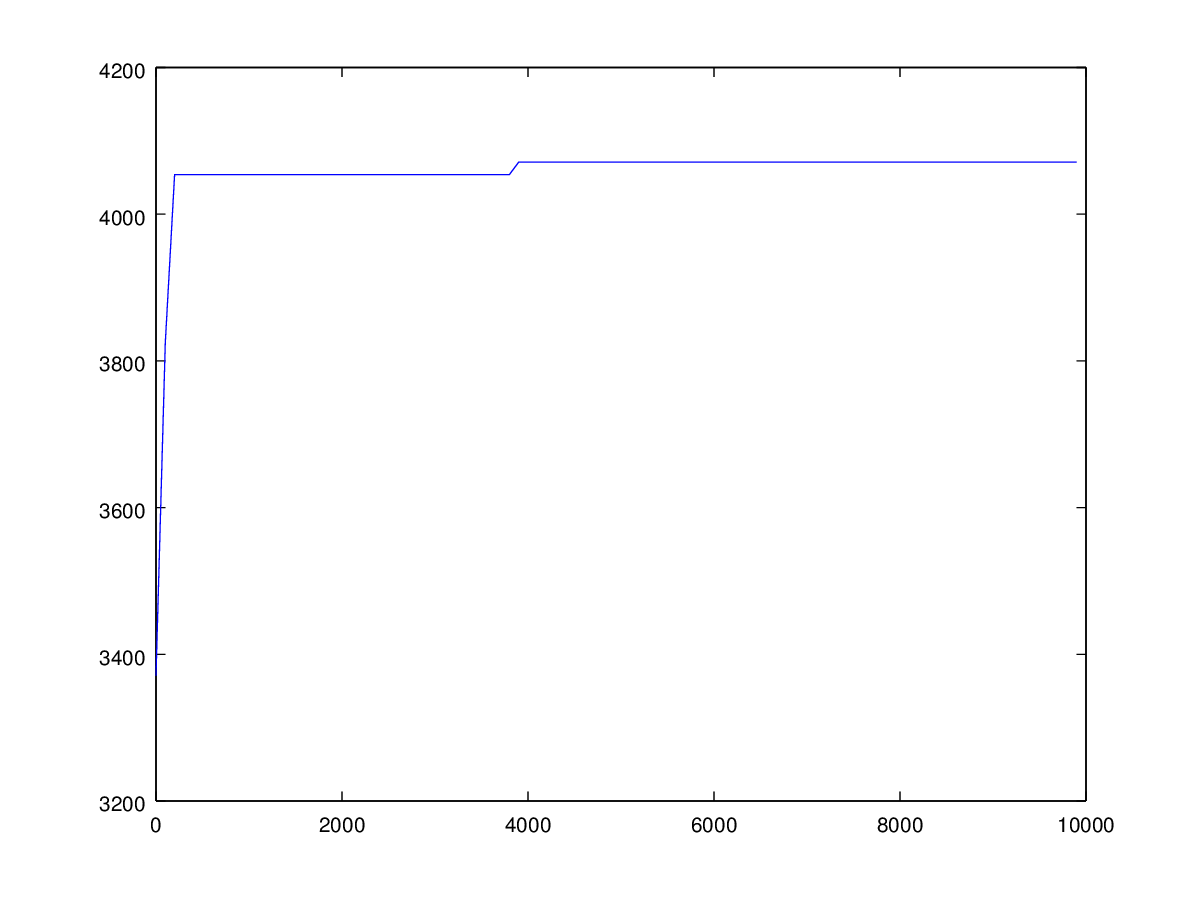
\includegraphics[width=0.5\textwidth]{images/graf_test_in.png}
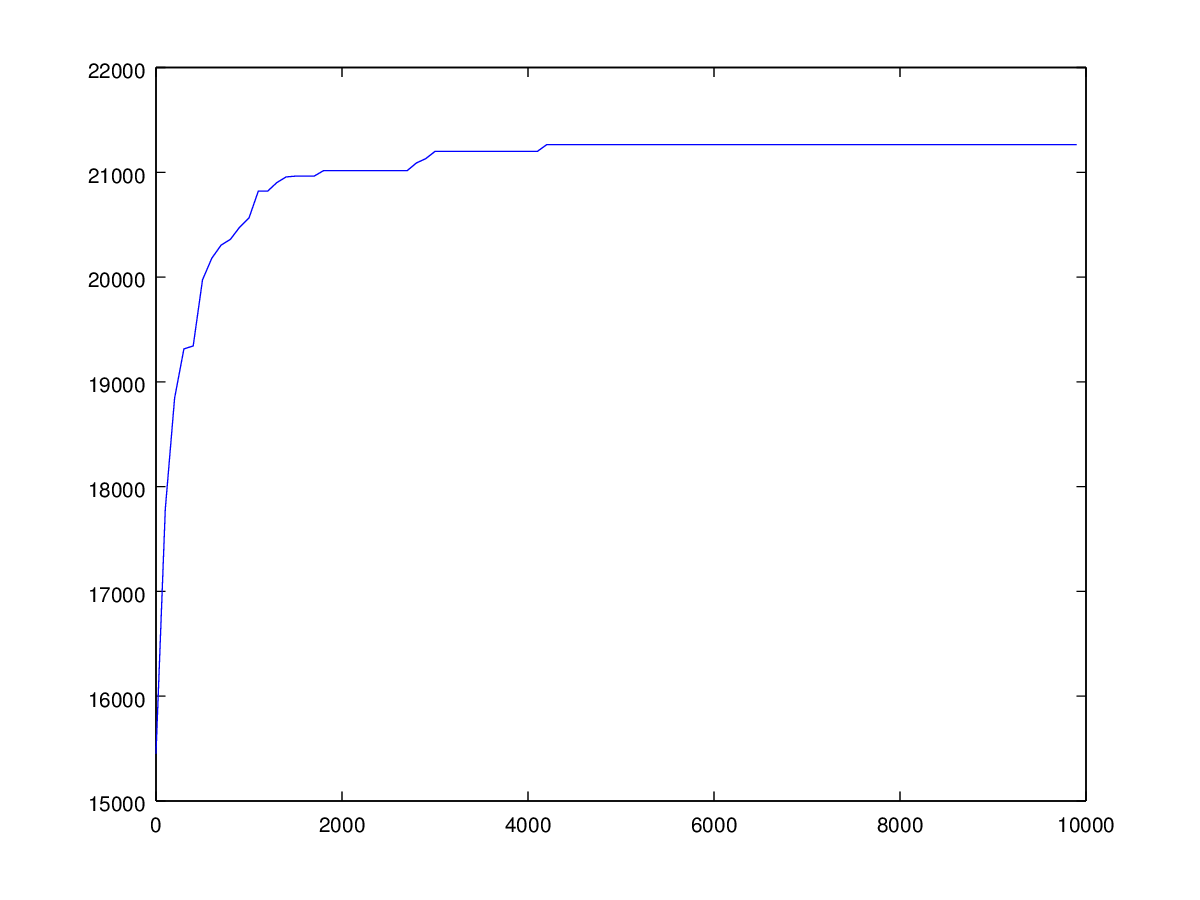
\includegraphics[width=0.5\textwidth]{images/graf_1.png}
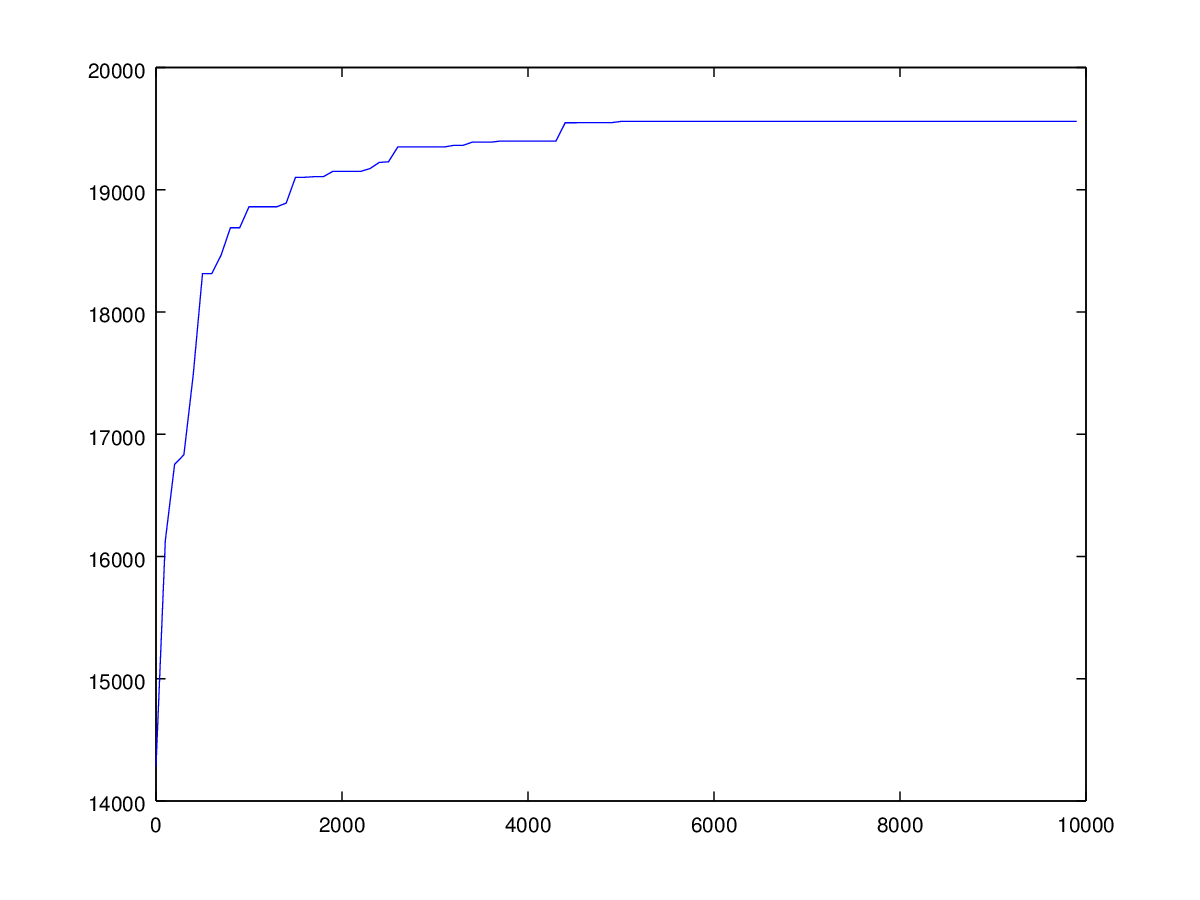
\includegraphics[width=0.5\textwidth]{images/graf_50.png}
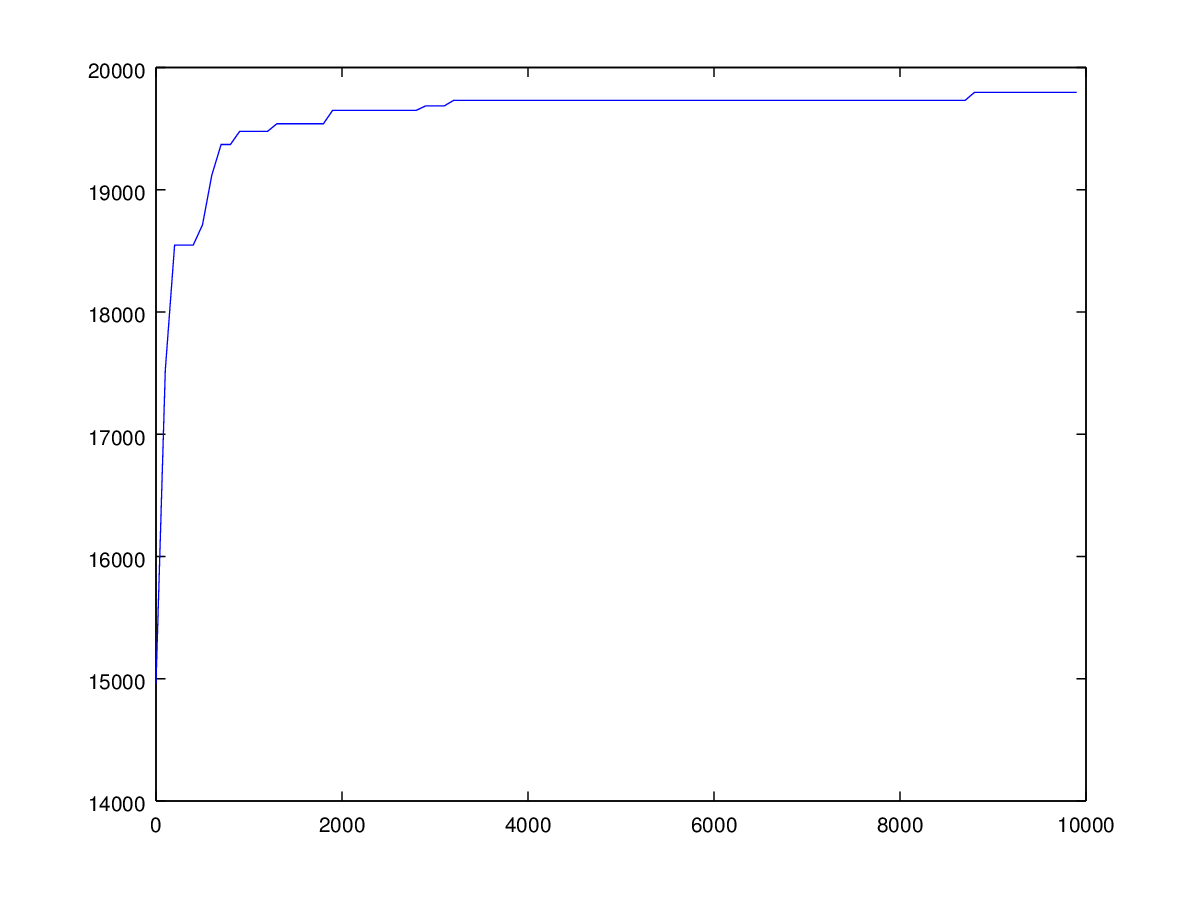
\includegraphics[width=0.5\textwidth]{images/graf_78.png}
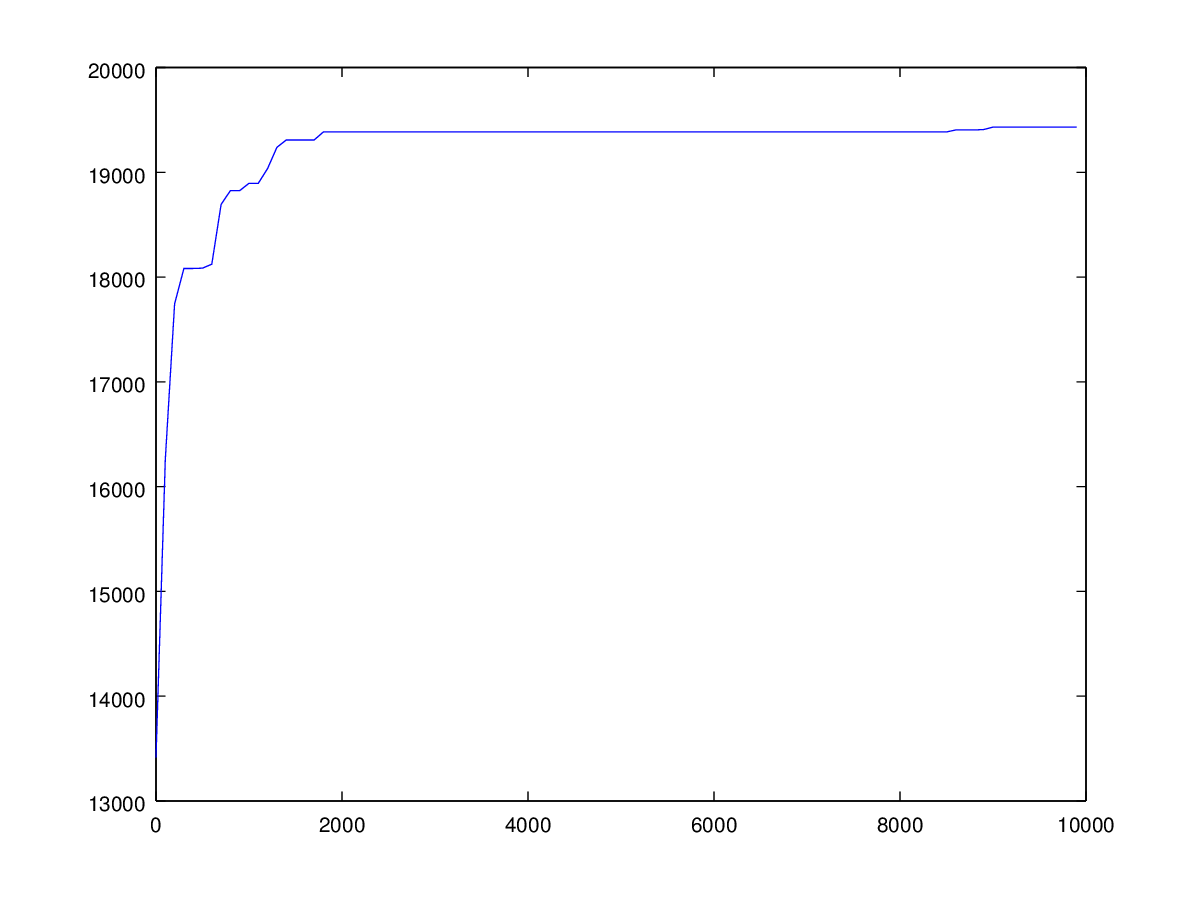
\includegraphics[width=0.5\textwidth]{images/graf_90.png}


% Puntos a tocar en el informe:
% 	Para el ejercicio 1:
% 		¿C\'ual fue la soluci\'on encontrada?
% 		¿Se encontr\'o m\'as de	una soluci\'on?
% 	Para el ejercicio 2:
% 		¿Qu\'e estrategia fue utilizada para el manejo de soluciones no factibles?

% *Probar variando los parametros (cantidad de poblaci\'on, mutaci\'on, escalara la funci\'on de fitness, velocidad de convergencia).
% *Explicar pq estamos usando elitismo (remplazo).
% *Hacer un algoritmo de fuerza bruta para hallar mejor soluci\'on en casos pequeños.
% 	Para tratar de responder si existe solucion y si hay mas de una.
% *Graficar fitness vs tiempo de ejecucion vs poblacion inicial.
% *Pensar en la distancia del espacio de busqueda.
% 	*Para generar una buena pob inicial.



	\section{Conclusi\'on}
	Al final de este laboratorio hemos podido decicir aquella librer\'ia que se adapta mejor a nuestras necesidades y que nos gustar\'ia usar para resolver el proyecto final. Adem\'as, en el proceso de realizaci\'on de este primer pr\'actico, logramos interiorizarnos en aspectos pr\'acticos y la aplicaci\'on de algoritmos gen\'eticos y la s\'intesis de informes con Latex y otras herramientas.


% ------ Final ------

	\bibliographystyle{IEEEtran}
	\bibliography{informe.bib}{}

\end{document}